\documentclass[final]{beamer}

\usetheme{RJH}
\usepackage[utf8]{inputenc}
\usepackage[frenchb]{babel}
\usepackage[orientation=portrait,size=a2,scale=1.2]{beamerposter}
\usepackage[absolute,overlay]{textpos}
\usepackage{url}
\usepackage[T1]{fontenc}

\usepackage{bbold}

\usepackage{wrapfig, blindtext}
\usepackage{ragged2e}

\usepackage{graphicx}
\usepackage{color}
\usepackage{hyperref}
\usepackage{amsmath}
\usepackage{amssymb}
\usepackage{pifont}
\newcommand{\cmark}{\ding{51}}%
\newcommand{\xmark}{\ding{55}}%
\usepackage[labelformat=empty]{caption}
\usepackage{framed}
%\usepackage{wrapfig}

\setlength{\TPHorizModule}{\paperwidth}
\setlength{\TPVertModule}{\paperheight}

\newcommand{\qedwhite}{\hfill \ensuremath{\Box}}

\definecolor{lightgreen}{rgb}{0.0,0.8,0.0}
\definecolor{lightblue}{rgb}{0.3,0.8,1.0}
\definecolor{lightred}{rgb}{0.874,0.180,0.105}
\definecolor{gray}{rgb}{0.4,0.4,0.4}
\definecolor{lightgray}{rgb}{0.8,0.8,0.8}
\definecolor{shadecolor}{rgb}{0.9,0.9,0.9}


\newenvironment{shaded2}{%
  \def\FrameCommand{\fboxsep=\FrameSep \colorbox{blue!20}}%
  \MakeFramed {\FrameRestore}}%
 {\endMakeFramed}


\title{Simple connectome inference from partial correlation statistics in calcium imaging}
\author{Antonio Sutera, Arnaud Joly, Vincent François-Lavet, Zixiao Aaron Qiu, Gilles Louppe, Damien Ernst and Pierre Geurts\\[1.5ex]
{\tiny
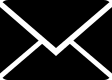
\includegraphics[scale=0.16]{images/mail.png}~\url{a.sutera@ulg.ac.be}
%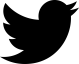
\includegraphics[scale=0.6]{images/twitter.png}~\href{https://twitter.com/glouppe}{@glouppe}

\includegraphics[scale=0.18]{images/github.png}~\url{https://github.com/asutera/kaggle-connectomics}
}}

\footer{}
\date{}

\makeatletter
\newcommand{\superimpose}[2]{%
  {\ooalign{$#1\@firstoftwo#2$\cr\hfil$#1\@secondoftwo#2$\hfil\cr}}}
\makeatother

\begin{document}
\begin{frame}{}


%% Abstract ------------------------------------------------------------------


\begin{textblock}{0.35}(0.01,0.115)


\begin{block}{Abstract \phantom{p}}

\vspace{-0.4cm}
\begin{center}

\begin{minipage}{0.95\linewidth}
\begin{shaded}
In this work, we propose \textbf{a simple yet effective solution} to the problem of
connectome inference in calcium imaging data. The proposed algorithm consists of
\textbf{two steps:
\begin{itemize}
\item[] {\color{lightgreen}i) processing the raw signals to detect neural peak activities,}
\item[] {\color{lightblue}ii) inferring the degree of association between neurons from partial
correlation statistics.}
\end{itemize}}
We summarises the methodology that led us to
win the Connectomics Challenge, proposes a simplified version of our method, and
finally compares our results with respect to other inference methods.

\end{shaded}
\end{minipage}
\end{center}

\end{block}


\end{textblock}


%% Context ------------------------------------------------------------

\begin{textblock}{0.62}(0.37,0.115)

\begin{block}{Context \phantom{p}}

Without being perfect, \textbf{calcium imaging} currently allows for \textbf{real-time and
simultaneous observation of neuron activity} from thousands of neurons,
producing \textbf{individual time-series representing their fluorescence intensity}.
From these data, the connectome inference problem amounts to retrieving the
synaptic connections between neurons on the basis of the fluorescence time-series. This problem is difficult to solve because of \textbf{experimental issues,
including
\begin{itemize}
\item[] {\color{lightgreen}i) masking effects (i.e., some of the neurons are not observed or
confounded with others),} 
\item[] {\color{lightblue}ii) the low sampling rate of the optical device with
respect to the neural activity speed,} or
\item[] {\color{lightred}iii) the slow decay of fluorescence.}
\end{itemize}}

\end{block}


\end{textblock}


%% Signal processing -----------------------------------------------------

\begin{textblock}{0.485}(0.01,0.26)

\begin{block}{Signal processing \phantom{p}}

Under the simplifying assumption that neurons are on-off units, characterised
by short periods of intense activity, or peaks, and longer periods of
inactivity, the first part of our algorithm consists of cleaning the raw
fluorescence data.
More specifically, time-series are processed using standard
signal processing filters in order to : 
\textbf{
\begin{itemize}
\item[] {\color{lightgreen}i) remove noise mainly due to fluctuations independent of calcium, calcium fluctuations independent of spiking activity, calcium fluctuations in nearby tissues that have been mistakenly captured, or simply by the imaging process ;}
\item[] {\color{lightblue}ii) to account for fluorescence low decay ; and}
\item[] {\color{lightred}iii) to reduce the importance of high global activity in the network.}
\end{itemize}}
\vspace{-2pt}

\begin{textblock}{0.485}(0.01,0.395)
\begin{minipage}{0.48\linewidth}
\begin{shaded}
\begin{center}
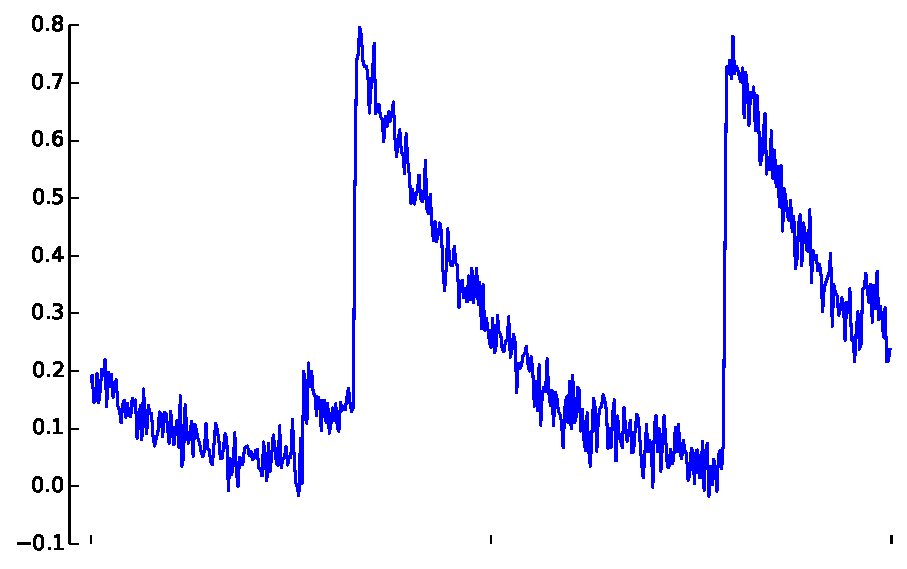
\includegraphics[width=0.85\linewidth]{images/original_curve.pdf}
\end{center}
\end{shaded}
\end{minipage}
\end{textblock}

\begin{textblock}{0.485}(0.25,0.395)
\begin{minipage}{0.48\linewidth}
\begin{shaded}
\vspace{15pt}
\hspace{1cm} {\small \textbf{Original curve}}
\vspace{30pt}
\end{shaded}
\end{minipage}
\end{textblock}

\begin{textblock}{0.485}(0.25,0.43)
\begin{minipage}{0.48\linewidth}
\begin{shaded2}
\begin{center}

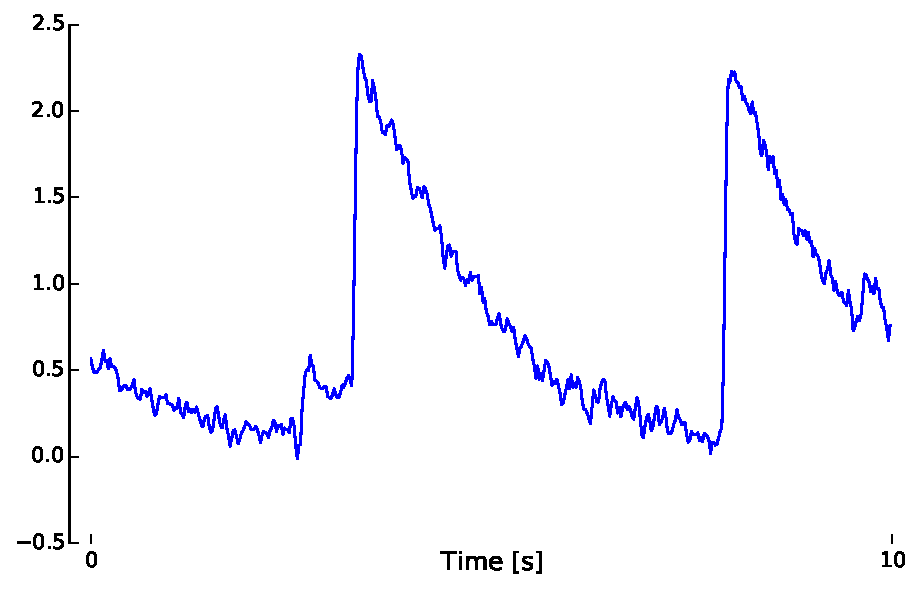
\includegraphics[width=0.85\linewidth]{images/filter_curve.pdf}
\end{center}
\vspace{15pt}
\end{shaded2}
\end{minipage}
\end{textblock}

\begin{textblock}{0.485}(0.01,0.495)
\begin{minipage}{0.48\linewidth}
\begin{shaded2}
\vspace{1pt}
{\color{lightgreen} \textbf{Applying a low-pass filter}}
\vspace{-5pt}
\begin{align*}
f_1(x^t_i) &= x^{t-1}_i + x^t_i + x^{t+1}_i,\\
f_2(x^t_i) &= 0.4 x^{t-3}_i + 0.6 x^{t-2}_i + 0.8 x^{t-1}_i + x_i^t.
\end{align*}
\vspace{-10pt}
\end{shaded2}
\end{minipage}
\end{textblock}

\begin{textblock}{0.485}(0.01,0.54)
\begin{minipage}{0.48\linewidth}
\begin{shaded}
\begin{center}

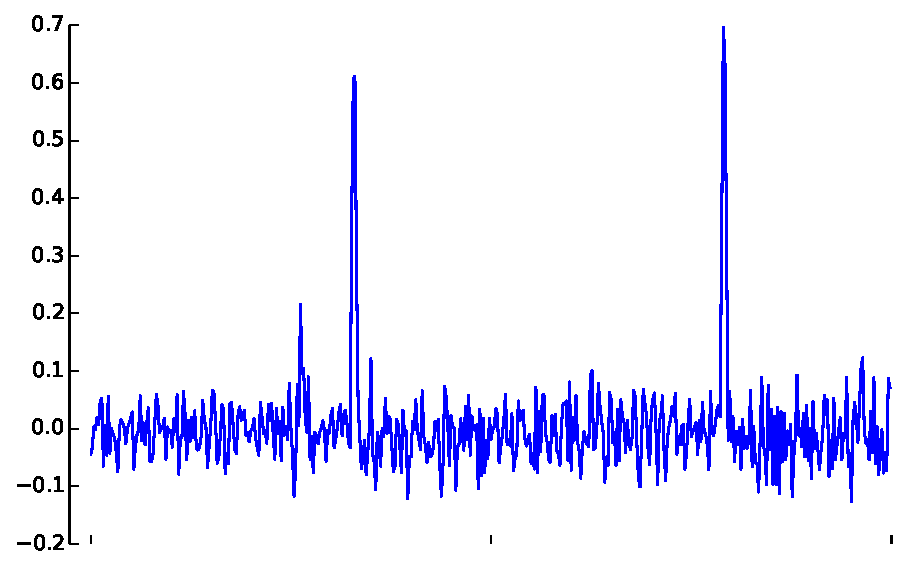
\includegraphics[width=0.85\linewidth]{images/diff_curve.pdf}
\end{center}
\end{shaded}
\end{minipage}
\end{textblock}

\begin{textblock}{0.485}(0.25,0.54)
\begin{minipage}{0.48\linewidth}
\begin{shaded}
\vspace{3pt}
{\color{lightgreen} \textbf{Applying a high-pass filter}}
\begin{align*}
g(x^{t}_{i}) = x^{t}_i - x^{t-1}_i,
\end{align*}
\vspace{5pt}
\end{shaded}
\end{minipage}
\end{textblock}

\begin{textblock}{0.485}(0.25,0.58)
\begin{minipage}{0.48\linewidth}
\begin{shaded2}
\begin{center}

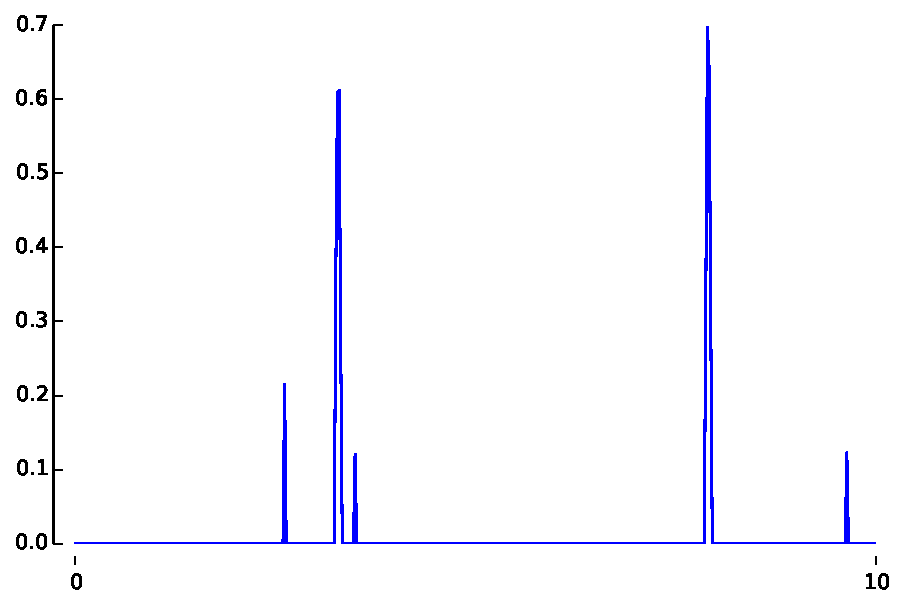
\includegraphics[width=0.85\linewidth]{images/threshold_curve.pdf}
\end{center}

\end{shaded2}
\end{minipage}
\end{textblock}

\begin{textblock}{0.485}(0.01,0.64)
\begin{minipage}{0.48\linewidth}
\begin{shaded2}
\vspace{7pt}
{\color{lightblue} \textbf{Applying a hard-threshold filter}}
\vspace{-5pt}
\begin{align*}
h(x^{t}_i) &= x^{t}_i \mathbb{1}(x^{t}_i \geq \tau) \text{ with } \tau > 0,
\end{align*}
\vspace{8pt}
\end{shaded2}
\end{minipage}
\end{textblock}


\begin{textblock}{0.485}(0.01,0.685)
\begin{minipage}{0.48\linewidth}
\begin{shaded}
\begin{center}
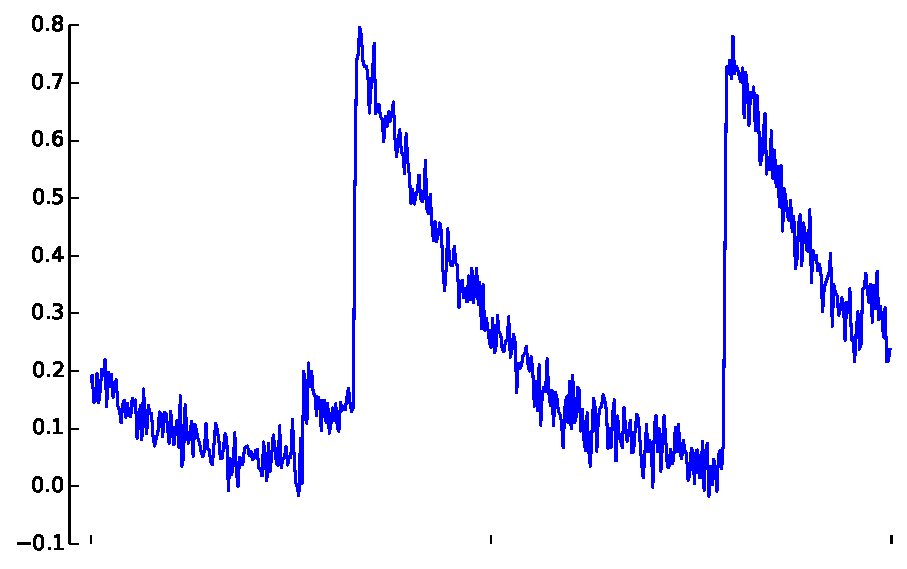
\includegraphics[width=0.85\linewidth]{images/original_curve.pdf}
\end{center}
\vspace{-14pt}
\end{shaded}
\end{minipage}
\end{textblock}

\begin{textblock}{0.485}(0.25,0.685)
\begin{minipage}{0.48\linewidth}
\begin{shaded}
\vspace{15pt}
{\color{lightred} \textbf{Magnify the importance of spikes that occur in cases of low global activity}}
\begin{align*}
w(x^{t}_i) = (x^{t}_i + 1 )^{1 + \frac{1}{\sum_{j} x^{t}_j}},
\end{align*}\vspace{42pt}
\end{shaded}
\end{minipage}
\end{textblock}



\end{block}







\end{textblock}





 

% \begin{columns}
% \begin{column}{0.01\linewidth}

% \end{column}
% \begin{column}{0.5\linewidth}
% 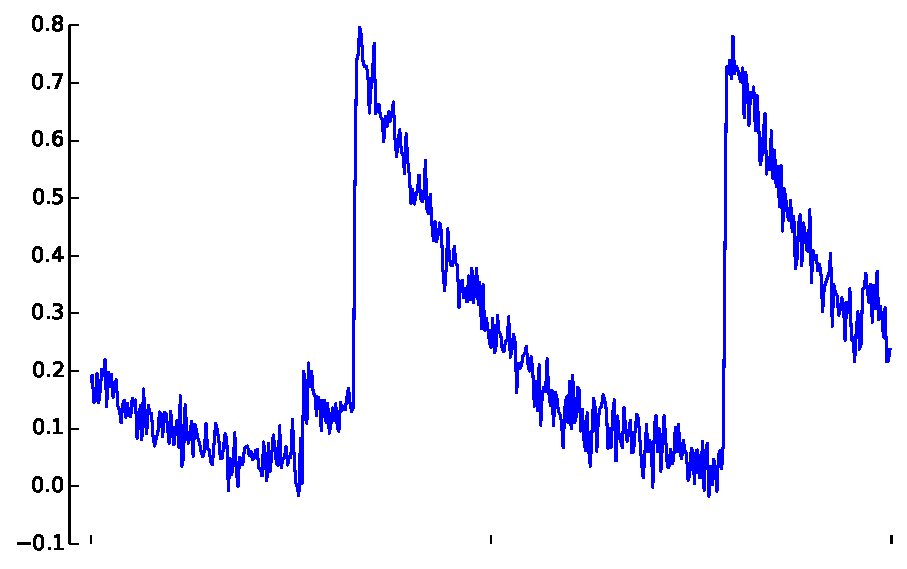
\includegraphics[width=0.9\linewidth]{images/original_curve.pdf}\\

% \begin{align*}
% f_1(x^t_i) &= x^{t-1}_i + x^t_i + x^{t+1}_i,\\
% f_2(x^t_i) &= 0.4 x^{t-3}_i + 0.6 x^{t-2}_i + 0.8 x^{t-1}_i + x_i^t.
% \end{align*}

% 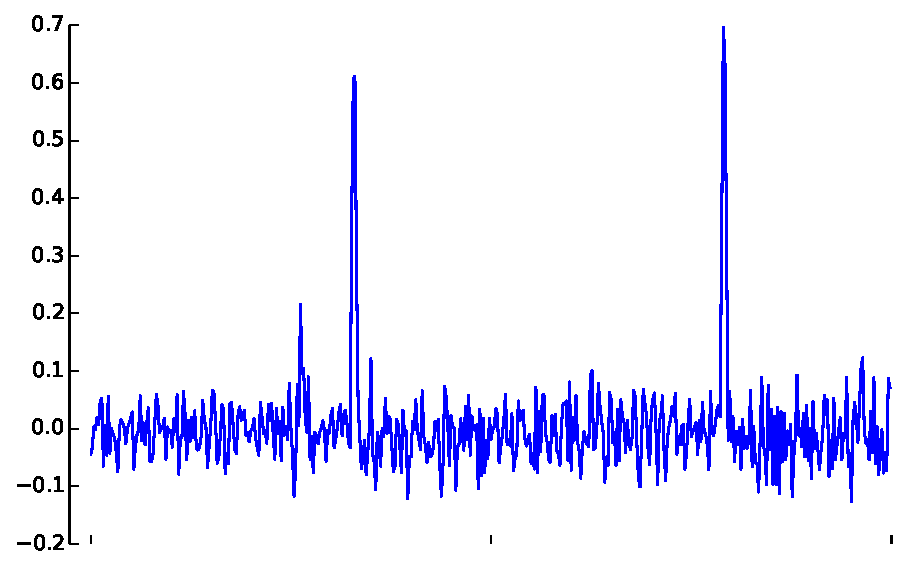
\includegraphics[width=0.9\linewidth]{images/diff_curve.pdf}\\[2ex]
% \begin{align*}
% h(x^{t}_i) &= x^{t}_i \mathbb{1}(x^{t}_i \geq \tau) \text{ with } \tau > 0,
% \end{align*}
% 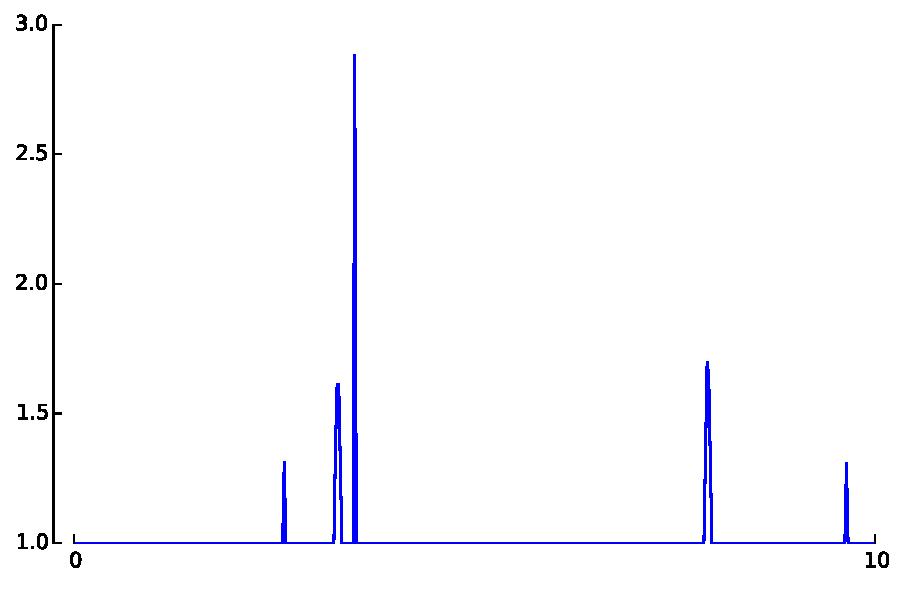
\includegraphics[width=0.9\linewidth]{images/weights_curve.pdf}\\

% \end{column}

% \begin{column}{0.5\linewidth}

% Original signal \\

% 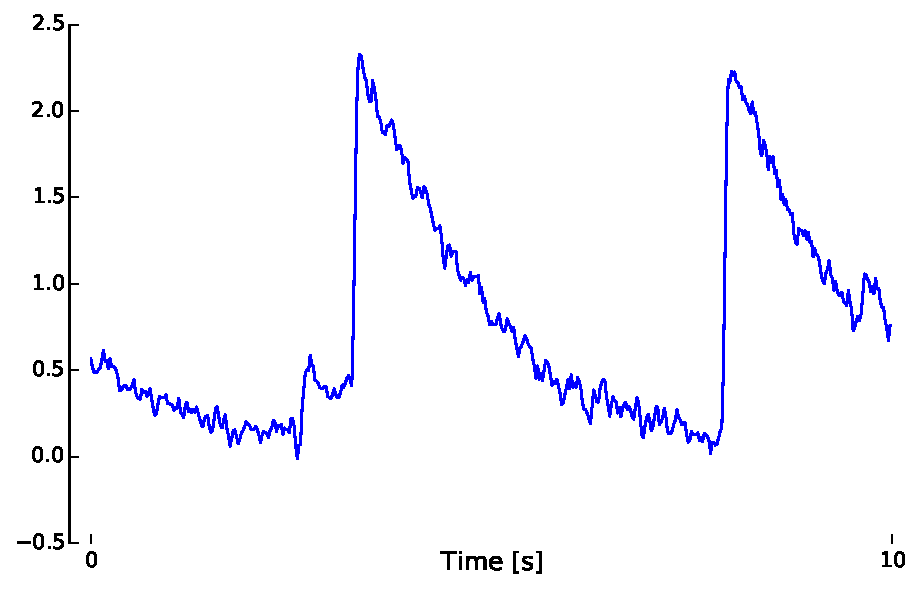
\includegraphics[width=0.9\linewidth]{images/filter_curve.pdf}\\[2ex]

% \begin{align*}
% g(x^{t}_{i}) = x^{t}_i - x^{t-1}_i,
% \end{align*}

% 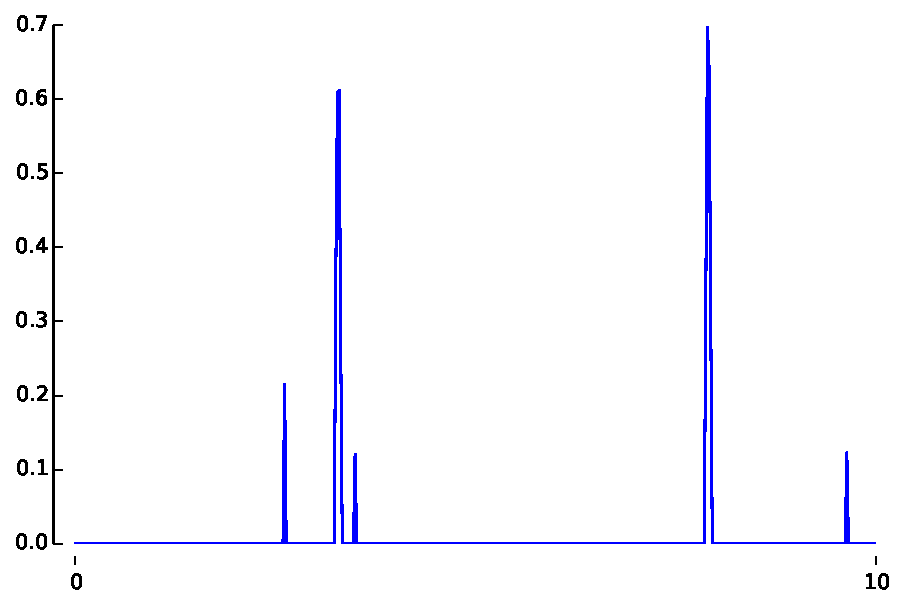
\includegraphics[width=0.9\linewidth]{images/threshold_curve.pdf}\\[2ex]

% \begin{align*}
% w(x^{t}_i) = (x^{t}_i + 1 )^{1 + \frac{1}{\sum_{j} x^{t}_j}},
% \end{align*}

% \end{column}
% \end{columns}

%% Connectome inference --------------------------------------------------

\begin{textblock}{0.485}(0.505,0.26)

\begin{block}{Connectome inference \phantom{p}}

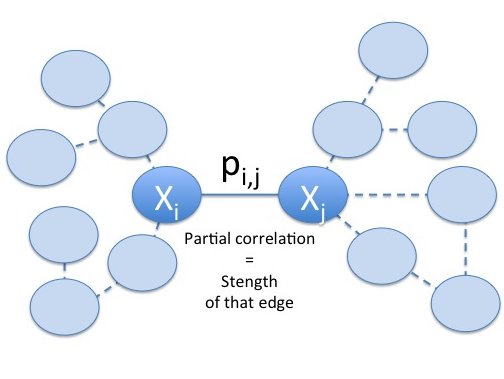
\includegraphics[width=\linewidth]{images/partial2.png}

Given the assumption of random variables drawn from the same time-invariant joint probability distribution, we then propose to use as a measure of the
strength of the connection between two neurons $i$ and $j$, the
\textit{Partial correlation} coefficient $p_{i,j}$ between their corresponding
random variables $X_i$ and $X_j$, defined by:

\begin{align*}
p_{i,j} =
-\frac{\Sigma^{-1}_{ij}}{\sqrt{\Sigma^{-1}_{ii} \Sigma^{-1}_{jj}}}, \label{eq:inverse}
\end{align*}
where $\Sigma^{-1}$, known as the precision or concentration matrix, is the inverse of the covariance matrix $\Sigma$ of $X$.\\ 

Assuming that the distribution $P_X$ is a multivariate Gaussian
distribution ${\cal N}(\mu,\Sigma)$, it can be shown that $p_{i,j}$ is
zero if and only if $X_i$ and $X_j$ are independent given all other
variables in $X$, i.e., $X_i \perp X_j|X^{-i,j}$ where $X^{-i,j}= X
\setminus\{X_i,X_j\}$.

\begin{itemize}
\item[{\color{green} \cmark}] Only direct associations
\item[{\color{green} \cmark}] Filter out spurious indirect effects
\item[{\color{green} \cmark}] Symmetric (i.e. $p_{i,j}=p_{j,i}$)\\[5ex]
\item[{\color{red} \xmark}] Edge orientation
\item[{\color{red} \xmark}] Sensitive to the value of parameters in the filtering process
\end{itemize}

\end{block}

\end{textblock}

%% Experiment ------------------------------------------------------------

\begin{textblock}{0.69}(0.01,0.78)

\begin{block}{Experiments \phantom{p}}

\vspace{-5pt}
\begin{wrapfigure}{r}{0.7\linewidth}
\centering
\tiny
\begin{tabular}{| l | c c c c | c c c c |}
\hline
& \multicolumn{8}{c|}{Performance with partial correlation}\\ \hline
& \multicolumn{4}{c|}{AUROC} & \multicolumn{4}{c|}{AUPRC} \\
with \textit{Method} $\backslash$ on \textit{normal-} & \textit{1} & \textit{2} & \textit{3} & \textit{4} & \textit{1} & \textit{2} & \textit{3} & \textit{4} \\
\hline
\hline
No  filtering       					& 0.777 & 0.767 & 0.772 & 0.774 & 0.070 & 0.064 & 0.068 & 0.072\\
$ h \circ g \circ f_1$                  & 0.923 & 0.925 & 0.923 & 0.922 & 0.311 & 0.315 & 0.313 & 0.304\\
$ w \circ h \circ g \circ f_1$          & 0.931 & 0.929 & 0.928 & 0.926 & 0.326 & 0.323 & 0.319 & 0.303\\
+ PCA         							& 0.932 & 0.930 & 0.928 & 0.926 & 0.355 & 0.353 & 0.350 & 0.333\\
Averaging           					& 0.937 & 0.935 & 0.935 & 0.931 & 0.391 &  0.390 &  0.385 & 0.375\\
Full method           					& \textbf{0.943} & \textbf{0.942} & \textbf{0.942} & \textbf{0.939} & \textbf{0.403} & \textbf{0.404} & \textbf{0.398} & \textbf{0.388}\\
\hline
PC & 0.886 & 0.884 & 0.891 &  0.877 & 0.153 & 0.145 & 0.170 & 0.132\\
GTE & 0.890 & 0.893 & 0.894 & 0.873 & 0.171 & 0.174 & 0.197 & 0.142\\
GENIE3 & 0.892 & 0.891 & 0.887 & 0.887 & 0.232 & 0.221 & 0.237 & 0.215 \\
\hline
\end{tabular}
\end{wrapfigure}

These results clearly show the importance of the filters and PCA (especially for AUPRC). Taking the average over
various parameter settings gives an improvement of 10\% in AUPRC but
only a minor change in AUROC. The last row (``Full method'') shows the
final performance of the method specifically tuned for the challenge
(see paper for all details). Although this
tuning was decisive to obtain the best performance in the challenge,
it does not significantly improve either AUROC or AUPRC.

Partial correlation and averaged partial correlation clearly outperform all other methods on all datasets. The
improvement is more important in terms of AUPRC than in terms of AUROC. As
expected, Pearson correlation performs very poorly in terms of AUPRC. GTE and
GENIE3 work much better, but these two methods are nevertheless clearly below
partial correlation.

\end{block}

\end{textblock}



%% Conclusion ------------------------------------------------------------

\begin{textblock}{0.28}(0.71,0.78)

\begin{block}{Conclusion \phantom{p}}
\vspace{-0.4cm}
\begin{center}

\begin{minipage}{0.95\linewidth}
\begin{shaded}

In this paper, we outlined a simple but efficient methodology for the problem
of connectome inference from calcium imaging data. Our approach consists of \textbf{two
steps: 
\begin{itemize}
\item[] {\color{lightgreen}i) processing fluorescence data to detect neural peak activities; and}
\item[] {\color{lightblue}ii) inferring the degree of association between neurons from partial 
correlation statistics.}
\end{itemize}}

Its simplified variant outperforms other
network inference methods while its optimized version proved to be the best method
on the Connectomics Challenge. Given its simplicity and good performance, we
therefore believe that the methodology presented in this work
would constitute a solid and easily-reproducible baseline for further work in
the field of connectome inference.
\end{shaded}
\end{minipage}
\end{center}

\vspace{-0.3cm}

\end{block}

\end{textblock}

\begin{textblock}{1}(0.01,0.99)
{\fontsize{12}{10}\textbf{Acknowledgments:}}
{\fontsize{8}{10}\textbf{A. Joly and G. Louppe are research fellows of the FNRS, Belgium. A. Sutera is a
recipient of an FRIA fellowship of FRS-FNRS, Belgium. This work is supported by
PASCAL2 and the IUAP DYSCO, initiated by the Belgian State, Science Policy
Office.}}
\end{textblock}

\end{frame}
\end{document}
